\chapter{Проведение космического эксперимента на научной аппаратуре «Плазменный кристалл-4»}
\label{cha:ch_3}
Научная аппаратура «Плазменный~кристалл~-~4» (НА~«ПК-4») была введена в эксплуатацию на борту
Международной космической станции (МКС) в июне 2015~года. Установка предназначена для экспериментального
исследования пылевой плазмы в условиях микрогравитации. В отличие от предыдущей научной аппаратуры
«ПК-3» и «ПК-3~Плюс», где пылевая плазма создавалась в емкостном радиочастотном (ВЧ) газовом разряде,
в НА~«ПК-4» пылевая плазма создается в однородном положительном столбе газового разряда постоянного тока (ПТ),
а также в индуктивном высокочастотном (ВЧ) разряде и в комбинированном ПТ/ВЧ разряде.

\section{Научная аппаратура «Плазменный~кристалл-4»}
\begin{figure}[t]
  \centering
  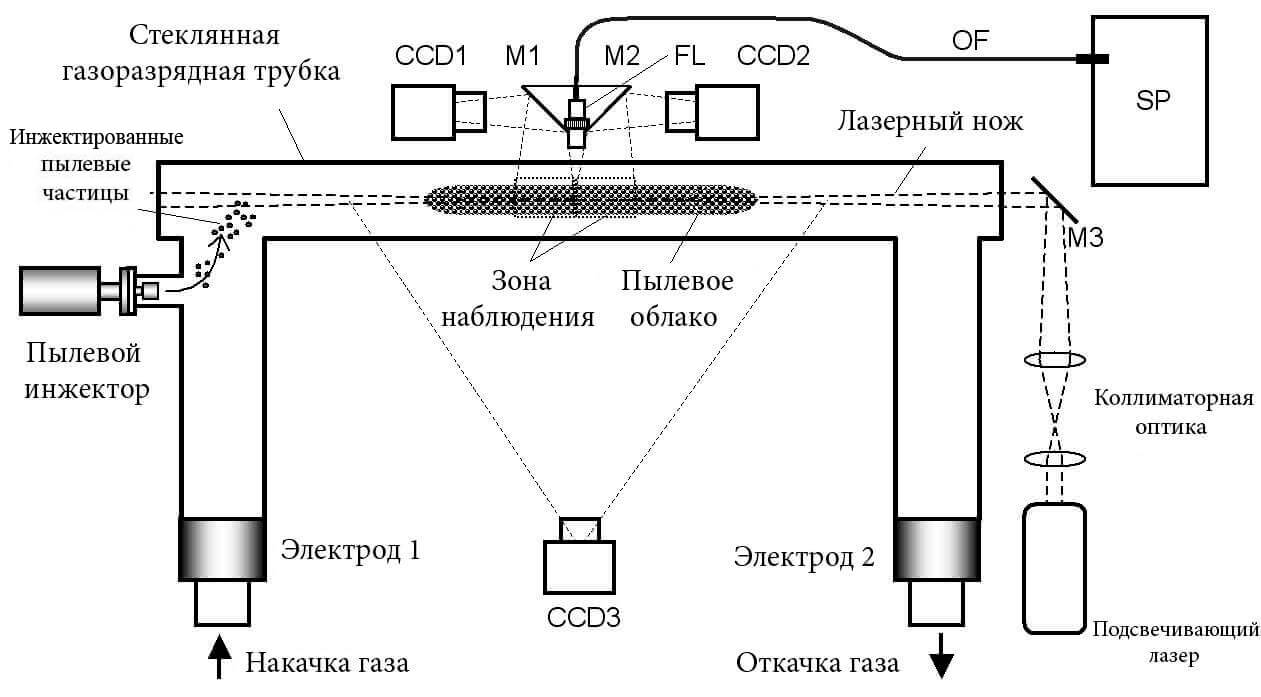
\includegraphics[width=12cm]{figures/fig31}
  \caption{Схема экспериментальной установки научной аппаратуры «Плазменный~кристалл-4». Здесь CCD1,~CCD2~--~камеры высокого разрешения;
           M1,~M2,~M3~--~зеркала; OF~--~оптоволоконный кабель; SP~--~спектрометр.}
  \label{fig:fig31}
\end{figure}

При исследовании влияния пылевой компоненты на спектр излучения плазмы газового разряда необходимо ввести
существенное количество пылевых частиц, чтобы эффект их влияния можно было измерить. Как правило, в лабораторных
установках по исследованию пылевой плазмы в разряде постоянного тока удается «подвесить» сравнительно небольшое
плазменно-пылевое облако размером порядка 1~см$^3$. Влияние такого облака на интенсивность спектральных линий
ненамного превышает ошибки измерений. Условия микрогравитации позволяют значительно увеличить размер облака,
усилить наблюдаемый эффект и аккуратно его измерить. Поэтому данный эксперимент проводился в
условиях микрогравитации на российско-европейской космической научной аппаратуре «Плазменный кристалл-4» \cite{Usachev-Elbrus}.

\begin{figure}[t]
    \begin{center}
         \subfloat[\label{sub:3D-scheme-pk4}]{
           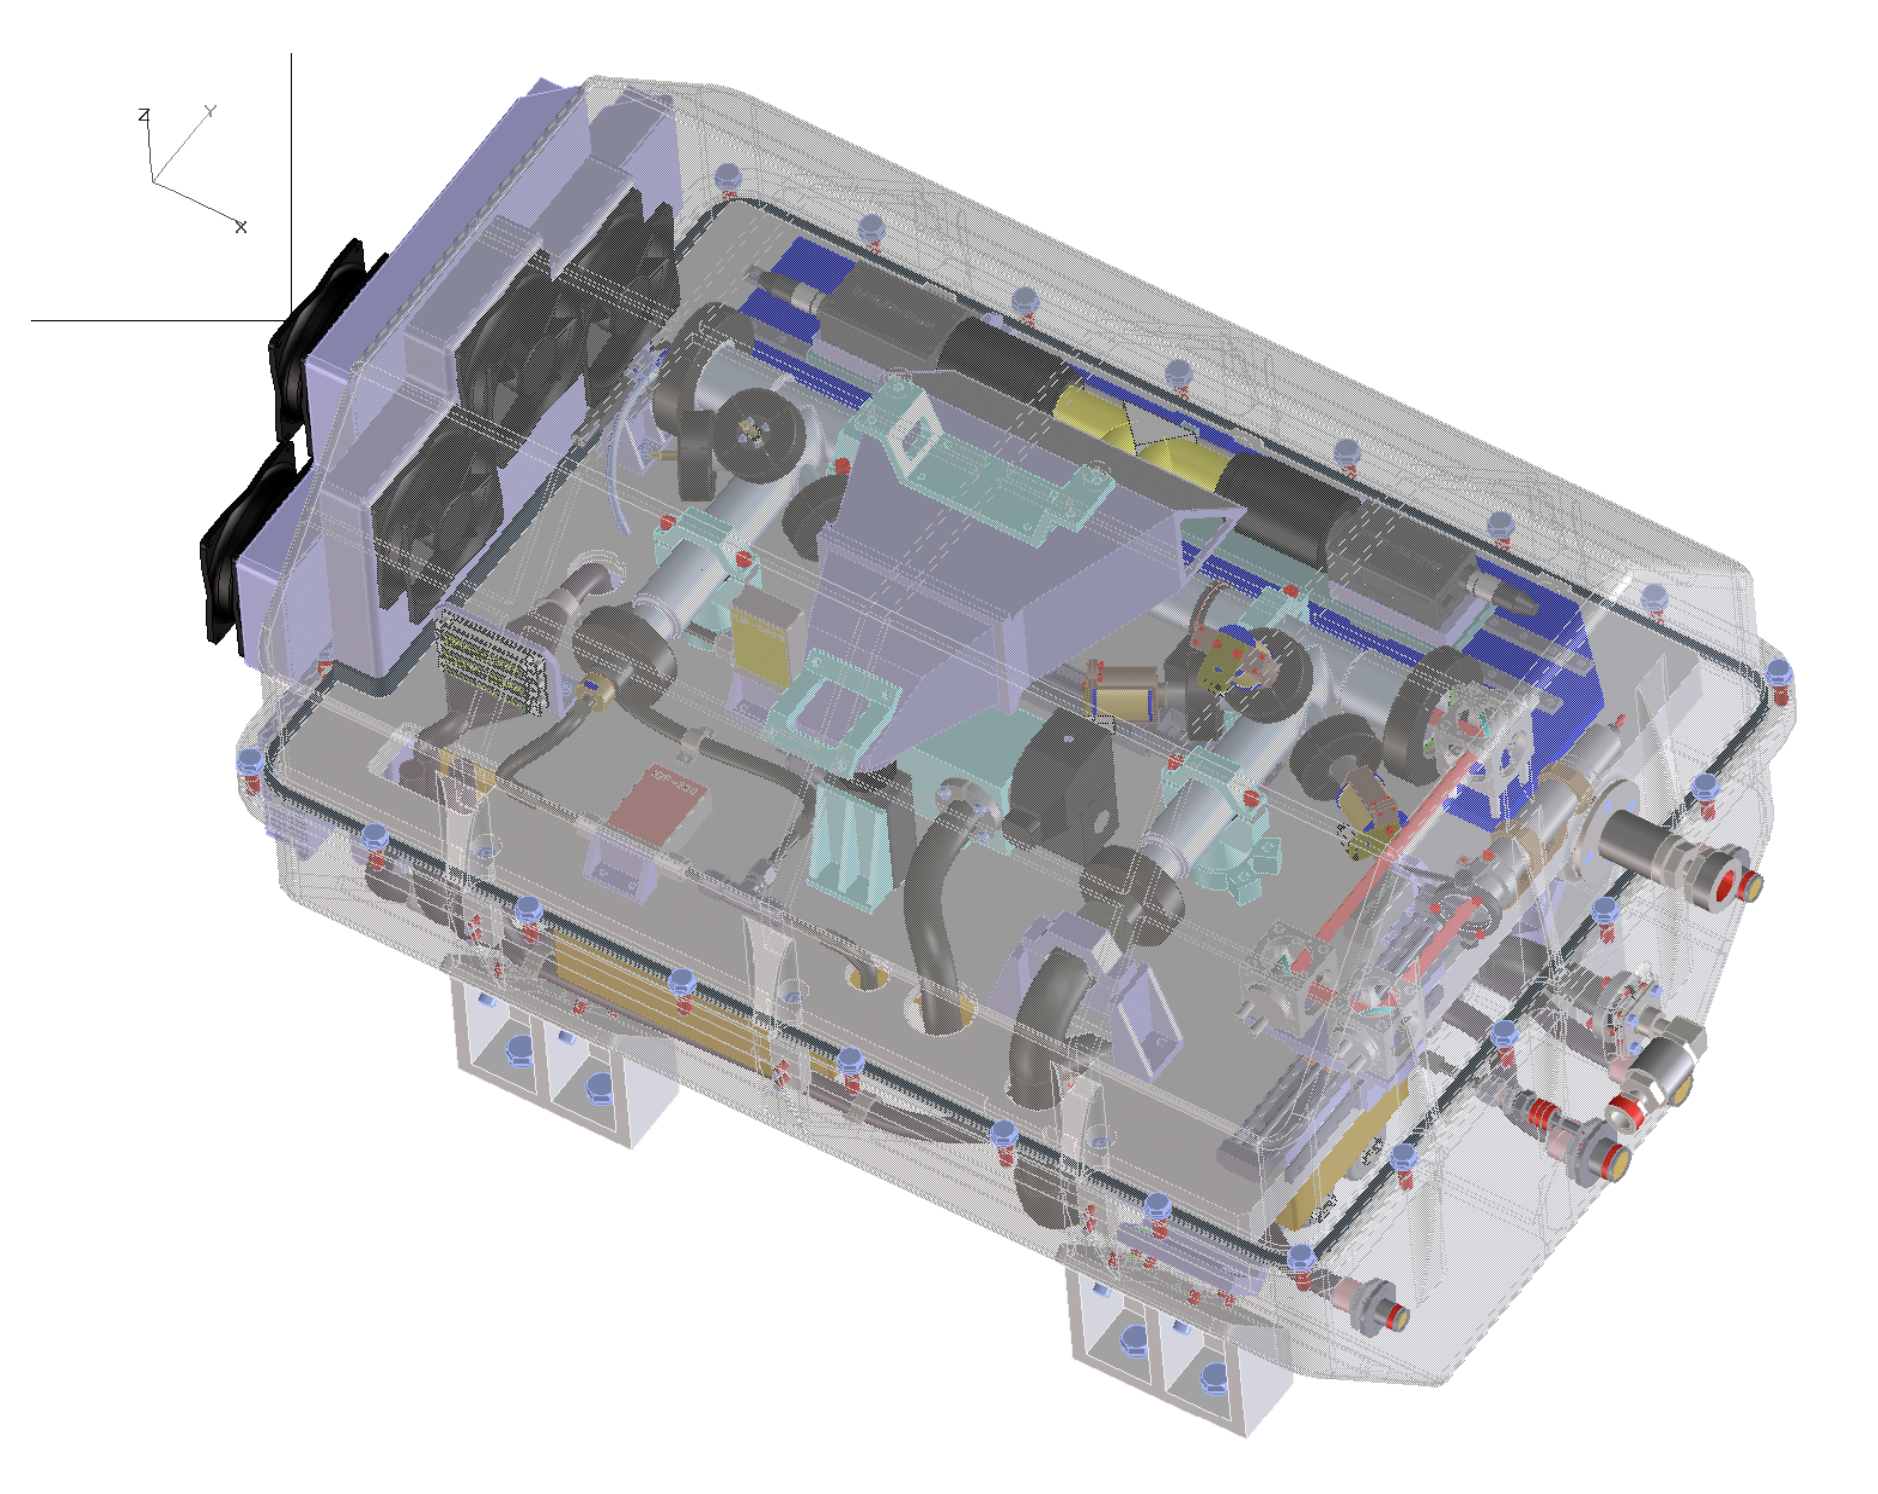
\includegraphics[width=0.45\textwidth]{figures/3D-scheme-pk4}
         }
         \subfloat[\label{sub:photo-pk4}]{
           \includegraphics[width=0.5\textwidth]{figures/photo-pk4}
         }
         \caption{Экспериментальная установка научной аппаратуры «Плазменный~кристалл-4»: \pt(а) 3D-модель внутренностей,
                  \pt(б) фото уже собранной установки в лабораторных условиях.}
    \label{fig:pk4}
    \end{center}
\end{figure}

\label{sec:sec_31}
Научная аппаратура «Плазменный кристалл-4» установлена в стандартную стойку европейского лабораторного модуля «Колумбс»
Международной космической станции (МКС). ОИВТ РАН является одной из организаций-поставщиков космического
эксперимента «ПК-4» (НА «ПК-4») и имеет доступ к постановке и проведению экспериментов.

Основой экспериментальной установки является П-образная стеклянная разрядная трубка с внутренним диаметром 30~мм
и общей длиной 85~см, которая заполнена атомарным неоном под давлением 60~Па.
На концах трубки установлены цилиндрические электроды из нержавеющей стали, которые используются для создания
и поддержания разряда постоянного тока. Системы вакуумной откачки и накачки газа соединяются с концами трубки
через данные электроды. Пылевые частицы подсвечиваются зеленым (532~нм) лазерным «ножом» и
регистрируются двумя камерами наблюдения высокого разрешения (CCD1 и CCD2).
Для отслеживания макро поведения подсвеченной плазмы используется общая камера наблюдения (CCD3) (см.~рисунок~\ref{fig:fig31}).

Каждая камера CCD1/CCD2 имеет поле зрения \math{22 × 17}$~мм\math{^2}$, разрешение \math{1600 × 1200}$~пикселей, а также
частоту кадросмен 35~кадров в секунду. Камеры дополняют друг друга, присоединяясь меньшими сторонами и имеют общий размер
\math{44 × 17}$~мм\math{^2}$. Эффективная полуширина лазерного «ножа» составляет 50~мкм в центре поля зрения,
а также 180~мкм по краям.

Камера CCD3 имеет возможность просматривать всю трубку целиком c разрешением \math{640 × 480}$~пикселей
и частотой 15~кадров в секунду. Используя калейдоскопическую систему, камера CCD3 также наблюдает плазменное свечение
в центральной части разрядной трубки через 3~спектральных фильтра: один серый фильтр с пропусканием 12\% и два узкополосных
помеховых фильтров, настроенных на 705 и 587~нм.

Одна из копий модифицированной экспериментальной установки НА~«ПК-4«, которая в собранном виде  внешне не имеет существенных отличий,
находится в институте ОИВТ РАН (см.~рисунок~\ref{fig:pk4}~\subref{sub:photo-pk4}).

\section{Спектрометр «OceanOptics~USB2000+»}
Для осуществления спектральной диагностики НА~«ПК-4» применяется модульный мини-спектрометр OceanOptics~USB2000+ (см.~рисунок~\ref{fig:full_usb2000+}).
В основе лежит 2048-пиксельная ПЗС-линейка, которая позволяет проводить спектральные измерения в диапазоне длин
волн 350-1100~нм со спектральным разрешением 1.5~нм. Приемная головка световода спектрометра устанавливается рядом
с камерами высокого разрешения (CCD1, CCD2) и подключается к спектрометру через оптическое волокно (см.~рисунок~\ref{fig:fig31}).
Время считывания одного спектра составляет 4~с. Данный спектрометр также подходит для осуществления
контроля чистоты плазмы во время экспериментов.
\begin{figure}[t]
    \begin{center}
         \subfloat[\label{sub:usb2000+}]{
           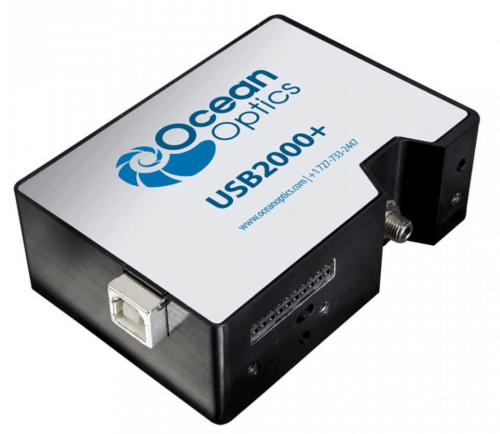
\includegraphics[width=0.47\textwidth]{figures/usb2000+}
         }
         \subfloat[\label{sub:cross_section_usb2000+}]{
           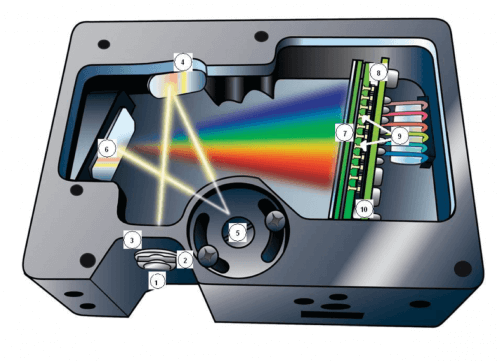
\includegraphics[width=0.47\textwidth]{figures/cross_section_usb2000+}
         }
         \caption{Модульный мини-спектрометр OceanOptics~USB2000+: \pt(а) внешний вид,
                  \pt(б) внутреннее устройство.}
    \label{fig:full_usb2000+}
    \end{center}
\end{figure}

\section{Ход эксперимента}
\label{sec:experiment}
Проведение эксперимента начинается с вакуумной откачки газоразрядной трубки. В течение 2~дней она откачивается
до давления высокого вакуума порядка \math{< 2 × 10^{-3}}$~Па, а затем заполняется неоном до рабочего давления разряда порядка 60~Па.
Ток разряда при этом составляет \math{I_{DC} = 1}$~мА. После заполнения рабочим газом, с катодной стороны разрядной
\begin{figure}[t]
  \centering
  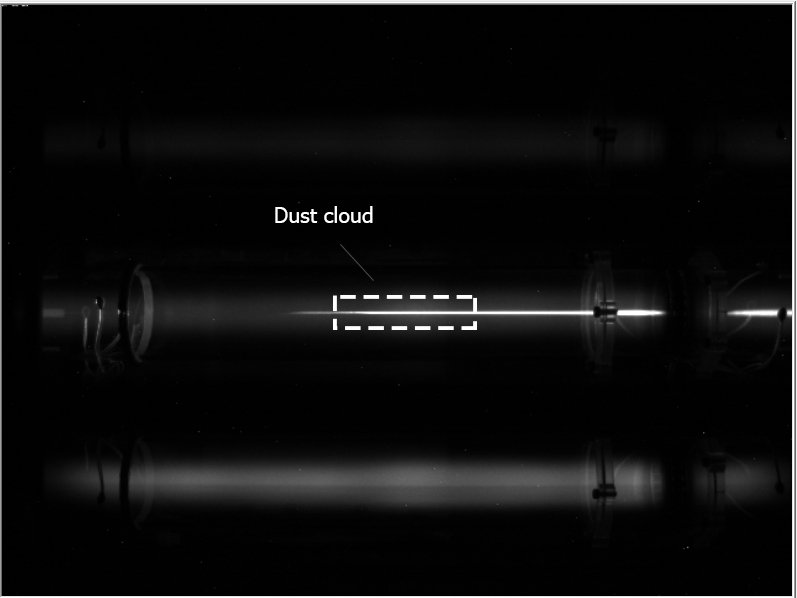
\includegraphics[width=14cm]{figures/common_camera}
  \caption{Кадр видеозаписи с общей камеры наблюдения в ходе эксперимента, отмеченная область пылевого облака явлется областью поля зрения
  камер высокого разрешения (CCD1, CCD2.}
  \label{fig:common_camera}
\end{figure}
трубки с помощью пылевого инжектора впрыскиваются монодисперсные пластические (меламиноформальдегидные) микросферы
(частицы пыли) с диаметром \marh{d~=~3.38 ± 0.07}~мкм. В силу высокой подвижности электронов пылевые частицы заряжаются
отрицательно и начинают оседать на стенках трубки. Для того, чтобы поддерживать баланс гибели и рождения и плавно
управлять положением пылевого облака, необходимо регулировать электрическое поле постоянного тока с помощью напряжения
между катодом и анодом. Наблюдая за пылевым облаком через общую камеру наблюдения CCD3,
облако переносится в центр трубки (см.~рисунок~\ref{fig:common_camera}), где за пылевыми частицами можно наблюдать с помощью
камер высокого разрешения CCD1 и CCD2, а также осуществлять спектральную диагностику излучения.

\begin{figure}[t]
  \centering
  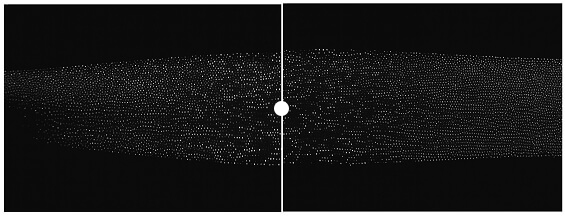
\includegraphics[width=16cm]{figures/high_resolution_cameras}
  \caption{Кадры видеозаписей с двух камер наблюдения высокого разрешения CCD1 и CCD2. Кадры синхронизированы во времени, а также пространственно дополняют друг друга.}
  \label{fig:high_resolution_cameras}
\end{figure}

Таким образом, для получения эксперимента с исследуемым эффектом необходимо задать медленное движение пылевого облака при
неизменном токе между катодом и анодом, а затем провести спектральную диагностику в следующих состояниях облака:
\begin{itemize}
\item пылевое облако еще не влетело в область спектральной диагностики;
\item центр пылевого облака находится в области спектральной диагностики, что детектируется на спектре насыщенной
линией 532~нм зеленого лазера, а также видеозаписями с сопоставлением времени измерения спектров;
\item край пылевого облака попадает в область спектральной диагностики;
\end{itemize}

Поскольку облако представляет собой вытянутую овальную структуру, то можно измерить ширину облака в области спектральной диагностики
и оценить зависимость отношения интенсивностей от ширины облака, что описано в главе 4. А сейчас рассмотрим какие данные
в сыром виде приходят с НА~«ПК-4».

\section{Экспериментальные данные}
\label{cha:ch_3_4}
В научной аппаратуре «Плазменный~кристалл-4» выделены следующие каналы получения экспериментальных данных,
которые были задействованы в какой-либо мере в данной работе:
\begin{enumerate}
    \item Видеозаписи с двух камер высокого разрешения CCD1 и CCD2 (см.~рисунок~\ref{fig:high_resolution_cameras}).
    Видеофайлы в сыром виде имеют формат «.avi» с размером 4~Gb/min от одной камеры. На данных записях хорошо
    различимы отдельные пылевые частицы, что позволяет отслеживать их траектории движения, а также наблюдать за
    их поведением в любой момент времени.

    \item Видеозаписи с общей камеры наблюдения. Представляют собой файлы в формате «.avi» с размером 0.3~Gb/min (см.~рисунок~\ref{fig:common_camera}).
    На этих видеозаписях видно трубку целиком вместе с подсвеченной пылевой плазмой, где можно отследить макро поведение
    облака, в отличие от камер CCD1 и CCD2.

    \begin{figure}[t]
      \centering
      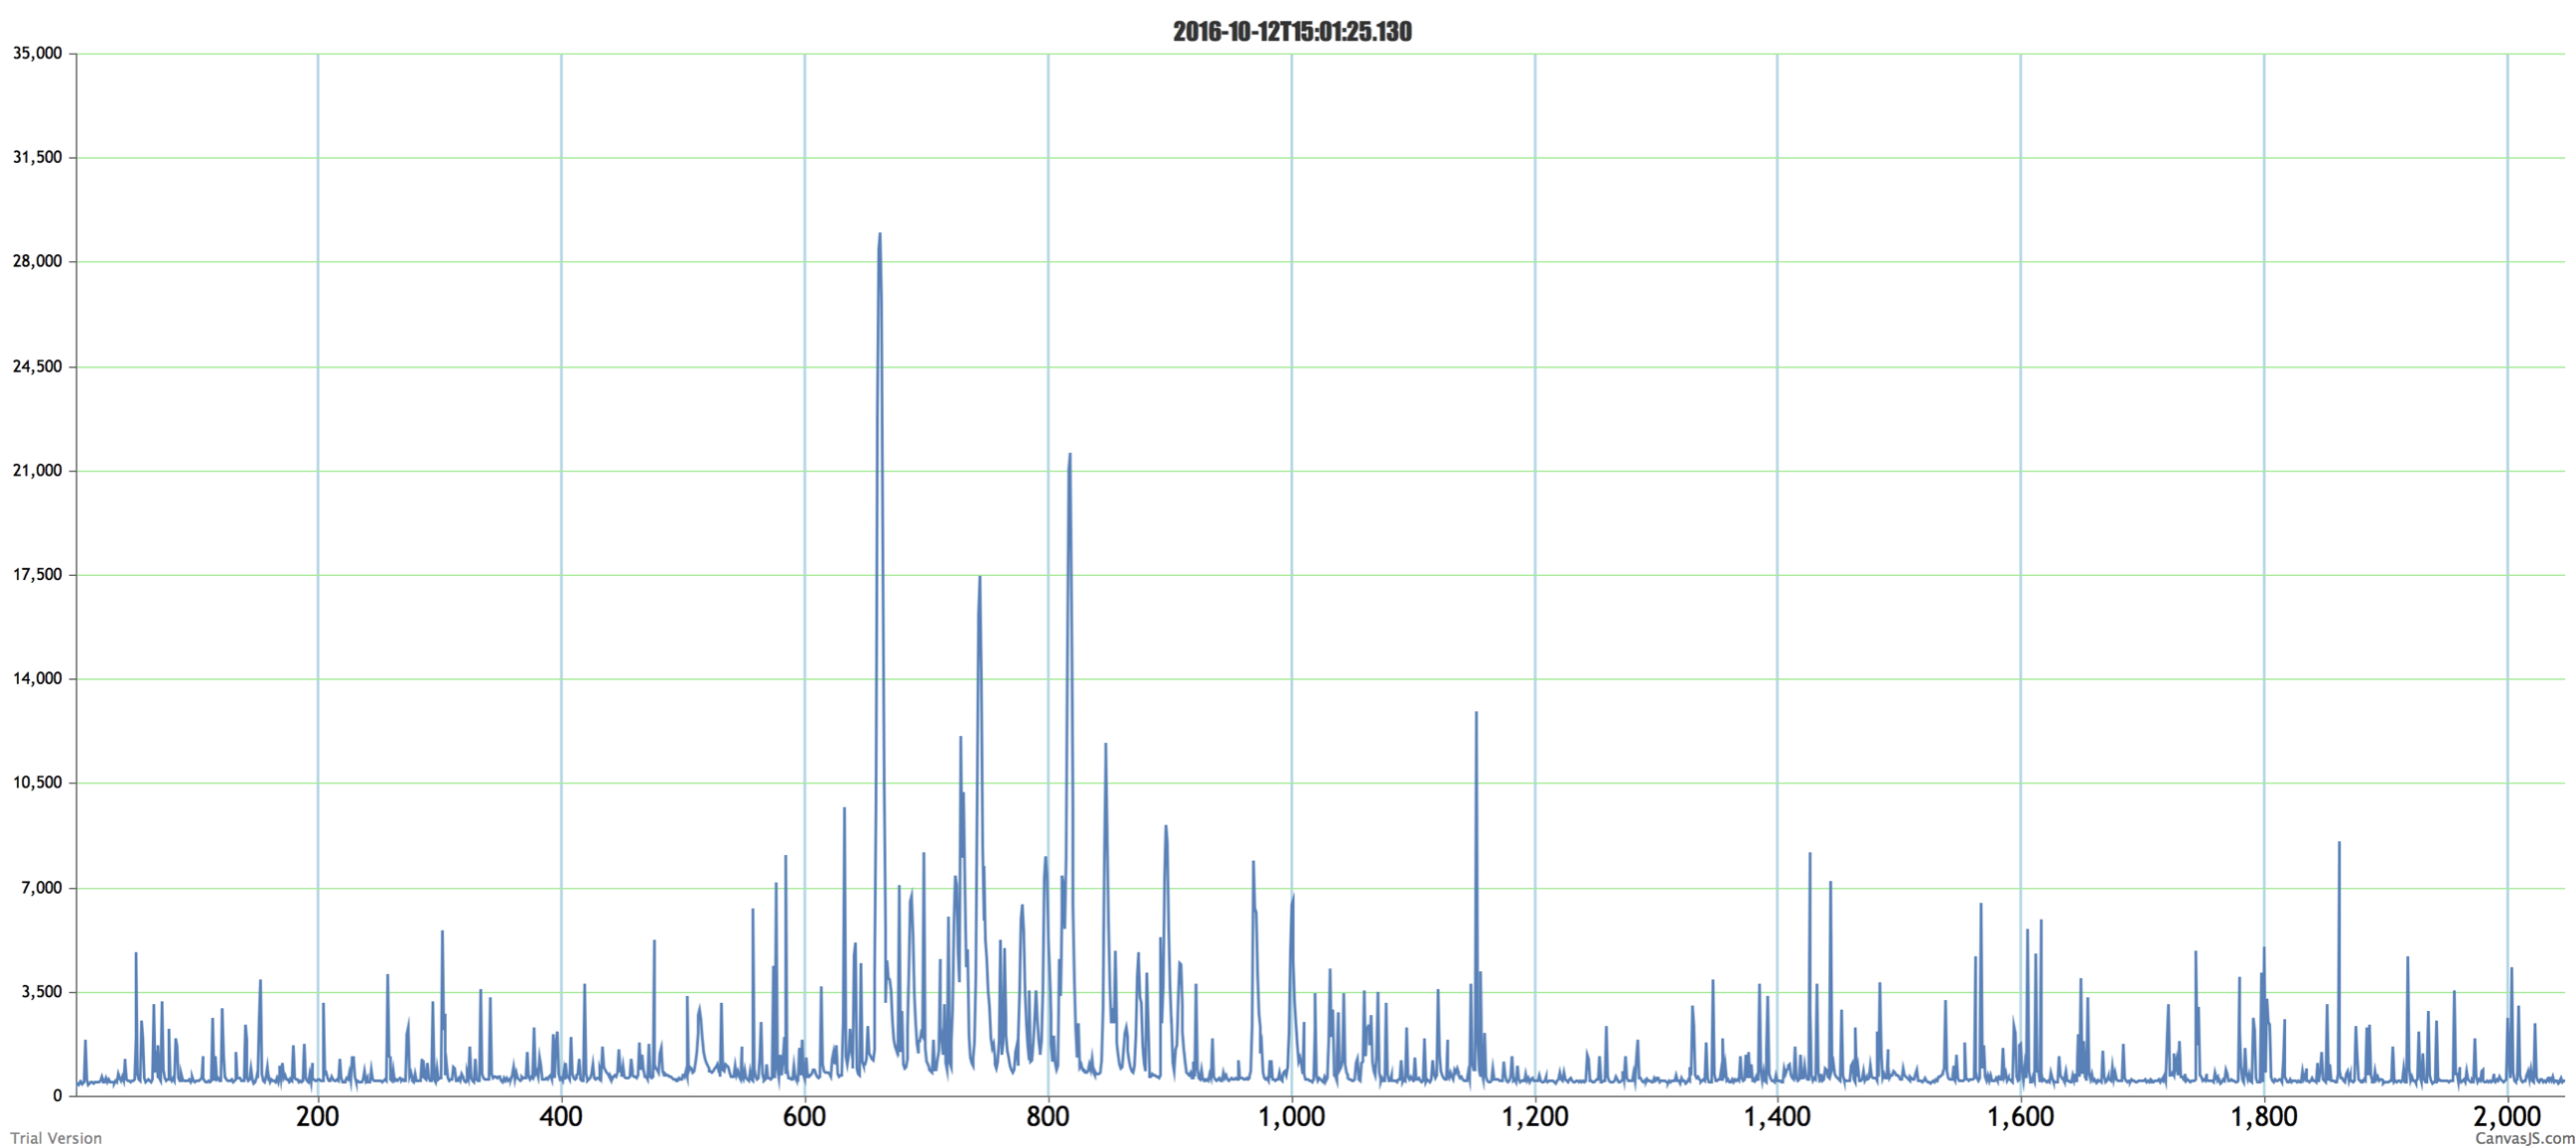
\includegraphics[width=16cm]{figures/raw_spectrum}
      \caption{Один из необработанных спектров эксперимента, полученных в ходе спектральной диагностики пылевого облака на НА~«ПК-4».}
      \label{fig:raw_spectrum}
    \end{figure}

    \item Спектральные данные. Представляют собой текстовые файлы в формате «.dat», которые имеют свою особую структуру
    по блокам, удобную для парсинга. Пример блока можно найти в \hyperref[app:app1]{приложении~А}. Эти спектральные данные
    хранят информацию о состоянии спектрометра в любой момент времени, его манипуляции, а также сырые данные с его ПЗС-линейки (см.~рисунок~\ref{fig:raw_spectrum}).

    \item Логи. Представляют собой текстовые файлы в формате «.log», которые содержат информацию обо всех
    технических изменениях в ходе эксперимента с временными отметками. Пример также можно найти в \hyperref[app:app2]{приложении~Б}.
\end{enumerate}
